\documentclass{article}

\usepackage{graphicx}
\usepackage{hyperref}
\usepackage[utf8]{inputenc}

\title{Relatório da segurança do SSL sobre dados}
\author{Nalbert Gabriel Melo Leal}
\date{13-10-2017}

\begin{document}

  \pagenumbering{gobble}

  \begin{figure}
		
\includegraphics[width=\textwidth]{imdLogo.png}
		\label{fig:imdLogo}
	\end{figure}

  \maketitle

  \newpage

  \tableofcontents
  \newpage

  \pagenumbering{arabic}

  \section{Introdução}

  \newpage

  \section{SSL}
  \subsection{Oque é SSL ?}
  \paragraph{}
  No ano de 1994 a Netscape criou um protocolo de segurança chamado SSL (secure
  socket layer) que cria um tunel lógico entre dois comutadores para que a
  comunicação entre eles não possa ser conpreendida por terceiros. Entenda o
  tunel lógico como uma comunicação sendo feita com uso de criptografia.
  \paragraph{}
    Esse canal criptografado entre é muito utilizado nos dias de hoje entre
  servidores e clientes para aumentar a segurança durante a troca de dados.
  Durante o acesso a um site para saber se existe o uso de SSL basta verificar
  se ao lado da URL da pagina existe o simbolo de um cadeado fechado, indicando
  uma conexão segura.

  \subsection{Como o SSL funciona ?}
  \paragraph{}
  O SSL como protocolo é bem simples. Para ativar o SSL em um sevidor é
  nescessário responder a algumas questões sobre identidade de quem esta sendo
  certificado (o servidor) e assim gerar um certificado que apos algum tempo
  definido irá ser invalidado.
  \paragraph{}
    Quando um servidor é requisitado por um cliente ele usa o certificado gerado
  para criar uma chave privada e uma publica. A chave privada vai servir para
  descriptografar os dados vindos do cliente, já a chave publica server para o
  cliente ter certza que a informação vem do servidor. Essas duas chaves permitem
  a troca de chaves unicas para que a comunicação atravez do canal criptografado
  possa acontecer.

  \subsection{É o SSL a prova de hackers ?}
    Já mencionamos que o SSL foi desenvolvido para aumentar a segurança entre
  cliente e servidor, entretanto isso não significa que seja inpossivel de
  burlar ou de descriptografar. Com pesquisas e com a insistencia de hackers é
  comum que em algum mommento se descubra vulnerabilidades.
  \paragraph{}
    No caso do SSL existe maneiras de se interceptar a comunicação no momento
  que ela esta sendo iniciada e assim interceptar os dados da comunicação. Esse
  metodo de invasão é chamado de "man in the middle", traduzido para "o homem
  no meio".
  \paragraph{}
    Esse ataque é potencialmente perigoso e permite que um atacante possa
  descobrir dados sensiveis de usuarios/servidor, sendo assim vamos demonstrar
  o quanto é fácil fazer um ataque "man in the middle" e como ele pode ser
  devastador, tanto para o usuário que pode ser colocado em grande risco e
  para o servidor, pois a baixa segurança pode fazer o numero de usuários cair.

  \newpage

  \section{Problemas do SSL}
  \paragraph{}
    Discutimos brevemente na sessão anterior um ataque que pode ocorrer ao SSL,
  mas esse não é o unico problema envolvendo o uso do SSL.

  \subsection{Prpblemas do SSL}
  \paragraph{}
  Se olharmos esse protocolo por sí só podemos achar que os motivos para não
  usa-lo são fracos, entretanto após olharmos um acumulo desse motivos podemos
  acabar vendo se vale ou não a pena usar.

  \begin{enumerate}
    \item O SSL causa um incremento no custo conputacional. Isso ocorre pois
    esse protocolo faz uso de criptografia, e a criptografia requer que sejam
    usados algoritimos custosos para encriptar e desencriptar.
    \item Aparentemente o SSL inpede que alguns tipos de cache, por exemplo o
    proxy transparente de ISP (Internet Service Provider ou em português
    Provedor de Serviço Internet). Com isso é nescessário um aumento no consumo
    de banda do servidor.
  \end{enumerate}

  \subsection{Como funcioan o ataque "man in the middle" ?}
  \paragraph{}
    Em uma coneção normal de troca e informações dois computadores trocam dados
  sem a interferência de terceiros. O termo "man in the middle" é uma referência
  a um ataque em que o atacante intercepta os dados entre duas pessoas (por
  exemplo o usuário e o facebook), registra esses dados e em alguns casos até
  os altera sem que as vítimas percebam.
  \paragraph{}
    Esse ataque claramente é extremamente perigoso por conta do atacante ter
  acesso aos dados que estão criptografados. Ocorre da seguinte forma:

  \begin{enumerate}
    \item O usuário faz uma requisição a um servidor.
    \item O atacante finge que é o servidor e assim intercepta a requisição.
    \item O atacante tem acesso aos dados do usuário em texto limpo.
    \item com esses dados pode-se fazer uma requisição ao servidor e receber
    a resposta.
    \item envia a resposta de volta ao usuario.
    \item usuário recebe a resposta e pensa que está em uma conexão segura.
  \end{enumerate}

  \subsection{O ataque "Man in the middle" e o SSL}
  \paragraph{}
  Como foi visto esse ataque é facil de se entender, a maneira como ele
  funciona com o SSL é igual com modificações para que o ataque funcione nesse
  protocolo. Com o SSL o atacante ao interceptar a conexão força um "downgrade"
  do HTTPS (HTTP sobre SSL) para HTTP e assim tem acesso aos dados do cliente
  em texto limpo, com isso pode fazer a conexão com o servidor e retornar a
  resposta ao usuário. Abaixo uma imagem:

  \begin{figure}[h!]
		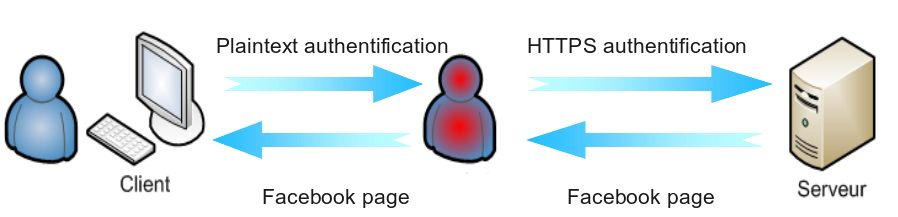
\includegraphics[width=\textwidth]{httpsManInTheMiddle.png}
		\label{fig:httpsManInTheMiddle}
	\end{figure}

    Na proxima sessão tem um passo-a-passo de como fazer o um ataque
  "man in the middle" e assim demonstrar que é um ataque completamente de
  ser executado com um conhecimento extremamente básico de redes de computadores
  possivel.

  \newpage

  \section{O experimento}
    Nessa sessão vamos demonstrar o quão facil é para interceptar dados SSL e
  assim ter acesso a dados dos usuários. Será tanbém demonstrado que o nivel de
  conhecimento nescessário é muito baixo, visto que usaremos ferramentas já prontas,
  assim podemos dizer que "lamers" podem facilmente fazer esse ataque, mostrando
  ser um ataque que nas mãos de hackers experientes pode acabar causando grandes
  danos ao serviço.

  \subsection{Requisitos}
    Os requisitos para fazer o experimento são os mesmos utilizados na hora
  da montagem para garantir que não averá problemas quando for replicado pelo
  leitor.

    \begin{enumerate}
      \item Usar o sistema operacional Ubuntu:
      \item Instalar as bibliotecas nescessárias com o comando:
        \$ sudo apt-get install build-essential ruby-dev libcap-dev net-tools
      \item Instalar a gema (software escrito na linguagem ruby) usando o
      gerenciador de pacotes "gem": \$ sudo gem install bettercap
      \item Possuir o programa "virtualbox" da oracle para rodar duas
      maquinas virtuais, uma será o servidor e a outra o cliente. Os links
      para baixar as maquinas estão abaixo (as maquinas virtuais
      já possuem os softwares nescessários para rodar o experimento):
      \begin{enumerate}
        \item Servidor:
        \item Cliente:
      \end{enumerate}
    \end{enumerate}

  \subsection{Passo-a-passo}

  \newpage

  \section{Conclusão}
  \subsection{Como se defender do "Man in the middle" sobre o SSL ?}
  \subsection{Considerações finais}

\end{document}
